\chapter{Quinn's Theorem}\label{c12}

Quinn\pageoriginale \cite{84} used Kirby's torus trick \cite{66} to verify the
stable version of the Connell-Hollingsworth conjecture. He then gave
an alternate proof of Ferry's thin $h$-cobordism theorem by the
method, due to Connell-Hollingsworth, given in the last lecture,
Namely, he proved the following result.

\begin{thm}\label{c12:thm12.1}
  Let $M^m$ be a closed (connected) smooth manifold (equi\-pped with a
  compatible metric $d(\,,\,)$) and let $\epsilon > 0$ be a real
  number. Then there exists a real number $\delta> 0$ such that any
  $\delta$-automorphism $f$ of a geometric group $G$ on $M$ is stably
  the composition of $m+1$ $\epsilon$-blocked automorphisms. That is,
  there exists a second geometric group $G_0$ such that the
  automorphism 
  $$
  f \oplus id_{g_0}: G \oplus G_0 \to G \oplus G_0
  $$
  can be factored as the compostition of $m+1$ $\epsilon$-blocked
  automorphisms of $G \oplus G_0$.
\end{thm}

This lecture and the next are devoted to proving Theorem
\ref{c12:thm12.1}. We start by introducing some notation. Let $A
\subset M$ be a subset and $G$ be a geometric group on $M$. Then
$G|_A$ is the geometric subgroup on $M$ generated by the basis
elements of $G$ in $A$. Note that $G=G|_A \oplus G|_{M-A}$. Let $i_A$
and $p_A$ be the inclusion $i_A : G|_A\to G$ and projection $p_A : G
\to G|_A$, respectively.

\begin{defi}\label{c12:defi12.2}
  An endomorphism $f: G\to G$ is a $\delta$-automorphism over $A$ if
  there exists an endomorphism $g: G \to G$ satisfying the following. 
  \begin{enumerate}
    \item Both $f$ and $g$ are $\delta$-endomorphisms.
      \item $p_A \circ f \circ g \circ i_A = id _{G\mid_{A}}= p_A
        \circ g \circ g\circ i_A$.
  \end{enumerate}
\end{defi}

If $A \subset M$, let $A^\delta= \{ x \in M \mid d(x, A)\leq
\delta\}$.

The next result follows directly from the definitions.

\begin{lemma}\label{c12:lem12.3}
  Let\pageoriginale $A^\delta \subset B$, $B^\delta \subset C$ and $C \subset M$. If
  $f: G \to G$ is a $\delta$-automorphism of a geometric group on
  $M$. Then $f \circ p_B: G_C \to G_C$ is a $\delta$-automorphism over
  $A$ where $G_C=G|_C$ is considered as a geometric group on $C$.
\end{lemma}

The key step in the proof of Theorem \ref{c12:thm12.1} is the
following lemma which Quinn proves by a variant of Kirby's torus
trick.

\begin{lemma}\label{c12:lem12.4}
  Fix an integer $n \geq 2$. Given $\epsilon > 0$, there exists a
  $\delta> 0$ such that the following is true for any geometric group
  $G$ on $\mathbb{D}^{n}$ and any $\delta'$-automorphism $f:G\to G$
  over $(2/3)\mathbb{D}^{n}$, where $\delta'\leq \delta$. There exists
  a second geometric group
  $H$ on $\mathbb{D}^n - \frac{1}{2} \mathbb{D}^n$ and a
  $\epsilon$-automorphism $\ob{f}: G \oplus H \to G \oplus H$ with
  $$
  \ob{f} |_{\frac{2}{5}\mathbb{D}^n}= f|_{\frac{2}{5}\mathbb{D}^n}.
  $$
\end{lemma}

\begin{rem}\label{c12:rem12.5}
  Let $\mathcal{G}=G \oplus H$. If $\epsilon + \delta' \leq
  \frac{1}{15}$, then $\ob{f}^{-1}\circ(f \oplus id_H): \mathcal{G}
  \to \mathcal{G}$ is blocked relative to the decomposition
  $$
  \mathcal{G} = \mathcal{G}\mid_{\frac{1}{3}\mathbb{D}^n} \oplus
  \mathcal{G}\mid_{\mathbb{D}^n- \frac{1}{3} \mathbb{D}^n} 
  $$
  and $\ob{f}^{-1} \circ (f \oplus id_{H})$ restricted to the 1st
  block is the identity map.
\end{rem}

\begin{figure}[H]
  \centering{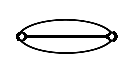
\includegraphics{vol86-figures/fig9.eps}\\
  Figure 9}
\end{figure}

Lemma\pageoriginale \ref{c12:lem12.4} will be proved in the next
lecture after we 
use it in this lecture to prove Theorem \ref{c12:thm12.1}. We start by
giving a first approximation to our proof and then discuss the
modifications needed to give a complete proof. Fix a handle body
docomposition of $M$ where each handle has diameter $\leq
\epsilon/4$. Such a handlebody can be constructed as dual to a
sufficiently fine trianglulation $K$ of $M$. See Figure 10.

\begin{figure}[H]
  \centering{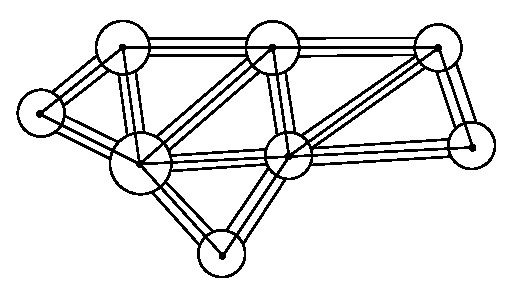
\includegraphics{vol86-figures/fig10.eps}\\
  Figure 10}
\end{figure}

Let $M_j=$ union of all the closed $i$-handles where $i \leq j$. We
can arrange, for each $j$-handle, an embedding
$$
h: (\mathbb{D}^j \times \mathbb{D}^{m-j}, S^{j-1} \times
\mathbb{D}^{m-j}) \to (M - \Int M_{j-1}, \partial M_{j-1})
$$
so that the following conditions are satisfied.
\begin{enumerate}
  \item Diameter (image $h$) $\leq \epsilon/2$.
    \item These embeddings have disjoint images.
      \item The $j$-handle $=h(\mathbb{D}^j \times \frac{1}{3}
        \mathbb{D}^{m-j})$.
\end{enumerate}

See Figure 11 for $j=1$. 
\begin{figure}[H]
  \centering{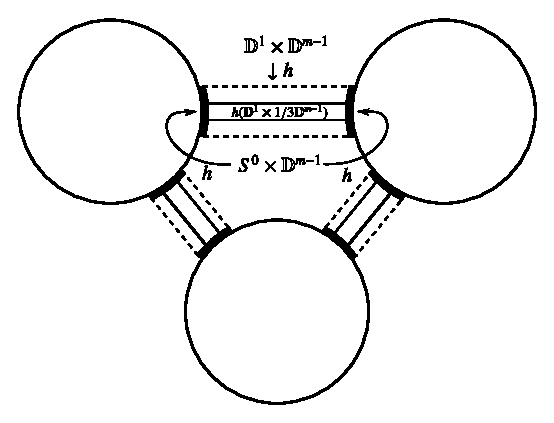
\includegraphics{vol86-figures/fig11.eps}\\
  Figure 11}
\end{figure}

Let\pageoriginale $f:G \to G$ be a $\delta_0$-automorphism of a
geometric group $G$ on $M$. We proceed to verify the conclusion of
\ref{c12:thm12.1} for $f$, provided $\delta= \delta_0$ is sufficiently
small. (How small will become evident from the proof and depends on
the handlebody structure just chosen.) First apply Lemma
\ref{c12:lem12.4} and Remark \ref{c12:rem12.5} to each 0-handle
independently. Hence there exists geometric group $G_0$, whose basis
is in $M- M_0$, such that 
$$
f_0 = f \oplus id: \mathcal{G}_0 = G \oplus G_0 \to \mathcal{G}_0
$$
is the composite map $\phi \circ \psi$ where $\phi$ is
$\epsilon$-blocked and $\psi$ is an $\epsilon_0$-automor\-phism of
$\mathcal{G}_0$ which is blocked relative to 
$$
\mathcal{G}_0 \mid_{M_0} \oplus ~\mathcal{G}_0 \mid_{M- M_0}
$$
and $\psi$ restricted to $\mathcal{G}_0 \mid_{M_0}$ is id. Let
$\psi_1$ denote the restriction of $\psi$ to $\mathcal{G}_0 \mid_{M-
  M_0}$. Then is suffices to show that $\psi_1$ is stably the
composition of $m$ $\epsilon$-blocked automorphisms over $M- \Int M_0$.

For each $1-$handle, $\psi_1$ restricted to $\mathbb{D}^1 \times
\frac{2}{2} \mathbb{D}^{m-1}$ (identifying via the embedding $h$) is a
$\delta_1-$automorphism over $\mathbb{D}^1 \times \frac{1}{2}
\mathbb{D}^{m-1}$. Projecting the basis for the geometric group
$\mathcal{G}_0 \mid_{\mathbb{D}^1 \times
  \mathbb{D}^{m-1}}$\pageoriginale to $\mathbb{D}^{m-1}$ gives a
$\delta_1$-automorphism over $\frac{1}{2} \mathbb{D}^{m-1}$. Applying
Lemma \ref{c12:lem12.4} and Remark \ref{c12:rem12.5} once again over
the transverse core (i.e., $\mathbb{D}^{m-1}$) of each 1-handle yields
a geometric group $G_1$ whose base is in $M - M_1$ and the following
factorization. Let
$$
\mathcal{G}_1 = \mathcal{G}_0\mid_{M- M_0} \oplus ~G_1 ~\text{and}~
f_1 = \psi_1 \oplus id_{G_1}: \mathcal{G}_1 \to \mathcal{G}_1,
$$
then $f_1$ is factored as the composite map $\phi_1 \circ \psi_1$
where $\phi_1$ is $\epsilon$-blocked and $\psi_1$ is an
$\epsilon_1$-automorphism of $\mathcal{G}_1$ which is blocked relative
to $\mathcal{G}_1 \mid_{M_1} \oplus ~\mathcal{G}_1 \mid_{M- M_1}$ and
$\psi_1$ restricted to $\mathcal{G}_1 \mid_{M_1}$ is id. The number
$\epsilon_1$ is determined by 
$$
\max \{ \diam h(\mathbb{D}^1 \times pt)\}
$$
and by $\ob{\epsilon}_1$ which is the number `$\epsilon$' used in this
application of Lemma \ref{c12:lem12.4}.

If we can continue this argument inductively to the 2-handles,
3-handles, $\ldots$, $(m-1)$-handles and $m$-handles, then we will
have proven Theorem \ref{c12:thm12.1}. But there are two weak points
which must be faced. First, if the diameters of the cores of the
1-handles are too large, i.e., the numbers diam $h(\mathbb{D}^1 \times
pt)$, then $\psi_1$ may not be sufficiently controlled to continue the
argument to the 2-handles. (And the same problem must be faced in
going from the 2-handles to the 3-handles, etc.) Quinn overcomes this
difficulty by carefully subdividing the original handlebody so that
the new cores of the handles $h (\mathbb{D}^j \times
\mathbb{D}^{m-j})$ all have ``very small'' diameter. This turns out
not to be too difficult to do once one has correct bookkeeping; i.e.,
once the notion of very small is made precise. See [84, p 330] for details.

The second difficult occurs in proceeding over the $(m-1)$-handles
since their transverse cores are $\mathbb{D}^1$ and Lemma
\ref{c12:lem12.4} is false for $\mathbb{D}^1$.\break ($A$ little thought
shows that the final step of proceeding over $m$-handles presents no
difficulty.) There are three ways around this. Quinn's meth\-od is by
introducing the notion of flux for a $\delta$-automorphism of
$\mathbb{D}^1$ over $\frac{1}{2} \mathbb{D}^1$. See [84 \S 8] for
details. On the other hand, the core of $M-\Int(M_{m-2})$ is a
1-complex and Connel-Hollingsworth \cite{20} proved their Conjecture
\ref{c10:conj10.3} for geometric groups on 1-complexes. Hence their
result can also be used to complete the argument.

The\pageoriginale third method uses that $\pi_1 (M- M_{m-2})$ is a
free group. It combines this fact with a vanishing result due to
Stallings \cite{91}; namely, $Wh(\Gamma)=0$ when $\Gamma$ is a free
group. Now the main argument, valid through the $(m-2)$-handles, shows
that $f$ stably factors as the composition of $m-1$ $\epsilon$-blocked
automorphisms $f_0, f_1, \ldots, f_{m-2}$ together with an
$\epsilon$-automor\-phism $\phi$ which is blocked relative to $M_{m-2}$
and $M- M_{m-2}$ and such that $\phi \mid_{M_{m-2}}=
id$. Consequently, $\hat{\phi}$ represemts 0 in $Wh (\pi_1 M)$ since
it is in the image of $Wh(\pi_1 (M - M_{m-2}))=0$. And Lemma
\ref{c9:lem9.3} yields the equation
$$
\hat{f} = \hat{f}_0 + \cdots + \hat{f}_{m-2} + \hat{\phi} 
$$
in $Wh (\pi_1M)$, provided $\epsilon < \ob{\delta}_0 /6m$ where
$\ob{\delta}_0$ denotes the number ``$\delta_0$'' fixed in Lecture
9. Furthermore, under this proviso each $\hat{f}_i=0$ by Lemma
\ref{c10:lem10.2}. Therefore, $\hat{f}=0$. Although this third method
does not prove Theorem \ref{c12:thm12.1}, it does establish the two
applications discussed in the Lectures \ref{c10} and \ref{c11};
namely, the topological invariance of Whitehead torsion and the thin
$h$-cobordism theorem.
